
\section{Tables and Figures}
\listoftables
\listoffigures
%introduction
\begin{sidewaystable}[hbpt]
 \centering
 \begin{tabularx}{\textwidth}{l l X }\toprule
\textbf{Attribute}              & \textbf{Attribute Type} &  \textbf{Attribute Range} \\\midrule
symboling               & ordinal     & -3, -2, -1, 0, 1, 2, 3 \\
\emph{normalized-losses}       & numerical   & continuous from 65 to 256\\
make                    & categorical & alfa-romero, audi, bmw, chevrolet, dodge, honda,
                               isuzu, jaguar, mazda, mercedes-benz, mercury,
                               mitsubishi, nissan, peugot, plymouth, porsche,
                               renault, saab, subaru, toyota, volkswagen, volvo\\
fuel-type               &categorical  &diesel, gas\\
aspiration              &categorical &std, turbo\\
num-of-doors            &ordinal & two, four\\
body-style              &categorical &hardtop, wagon, sedan, hatchback, convertible\\
\emph{drive-wheels}            &categorical &4wd, fwd, rwd\\
engine-location         &categorical &front, rear\\
\emph{wheel-base}              &numerical &continuous from 86.6 120.9\\
\emph{length}                   &numerical &continuous from 141.1 to 208.1\\
\emph{width}                    &numerical &continuous from 60.3 to 72.3\\
\emph{height}                   &numerical &continuous from 47.8 to 59.8\\
\emph{curb-weight}              &numerical &continuous from 1488 to 4066\\
engine-type             &categorical &dohc, dohcv, l, ohc, ohcf, ohcv, rotor\\
num-of-cylinders        &ordinal &two, three, four, five, six, eight, twelve\\
\emph{engine-size}              &numerical &continuous from 61 to 326\\
fuel-system             &categorical &1bbl, 2bbl, 4bbl, idi, mfi, mpfi, spdi, spfi\\
\emph{bore}                    &numerical &continuous from 2.54 to 3.94\\
\emph{stroke}                  &numerical &continuous from 2.07 to 4.17\\
\emph{compression-ratio}       &numerical &continuous from 7 to 23\\
\emph{horsepower}              &numerical &continuous from 48 to 288\\
\emph{peak-rpm}                &numerical  &continuous from 4150 to 6600\\
\emph{city-mpg}                &numerical & continuous from 13 to 49\\
\emph{highway-mpg}             &numerical &continuous from 16 to 54\\
\emph{price}                   &numerical &continuous from 5118 to 45400\\
\bottomrule
 \end{tabularx}
\caption{Description of \emph{autos} dataset.}
\label{tab:description_autos}
\end{sidewaystable}

\begin{figure}[hbpt]
 \centering
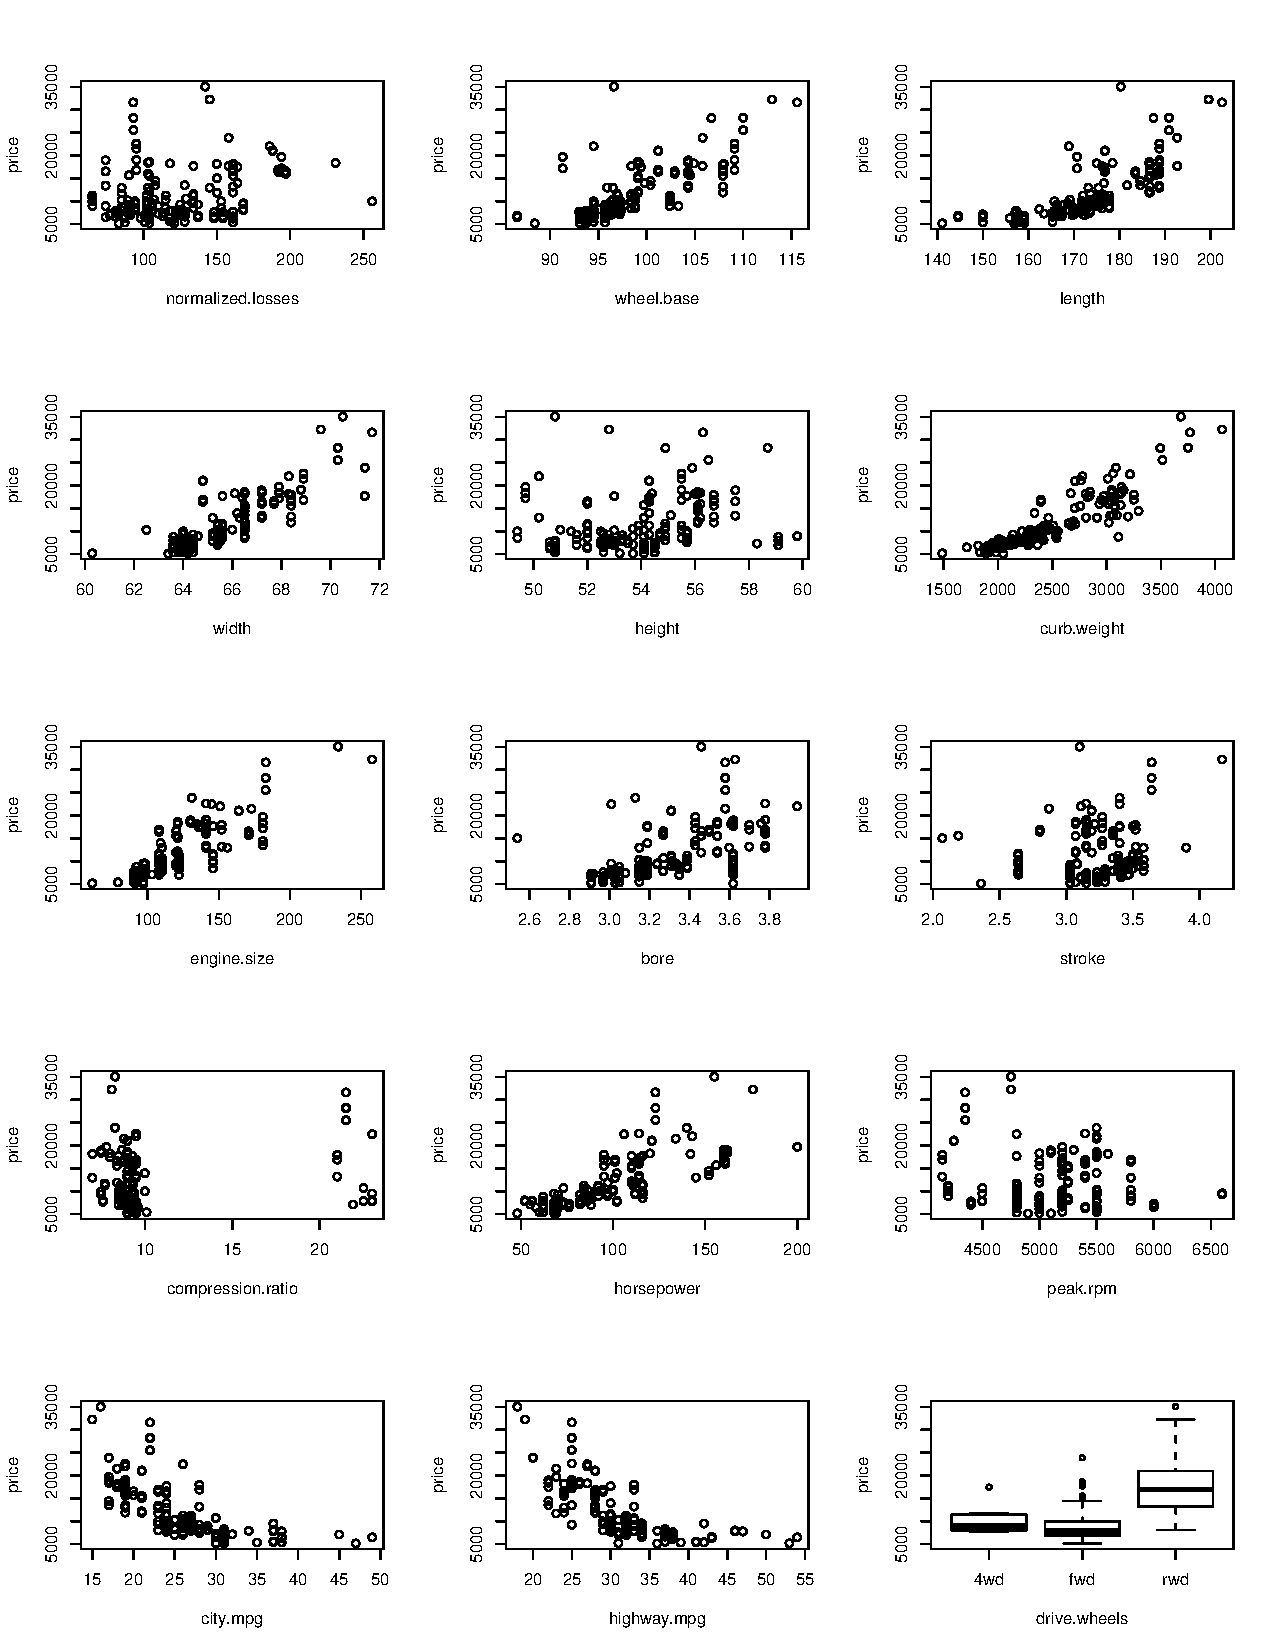
\includegraphics[width=\textwidth]{priceVsAllNum}
\caption{Response variable `price' versus regressors.}
\label{fig:priceVsAllNum}
\end{figure}

\begin{figure}[hbpt]
\centering
 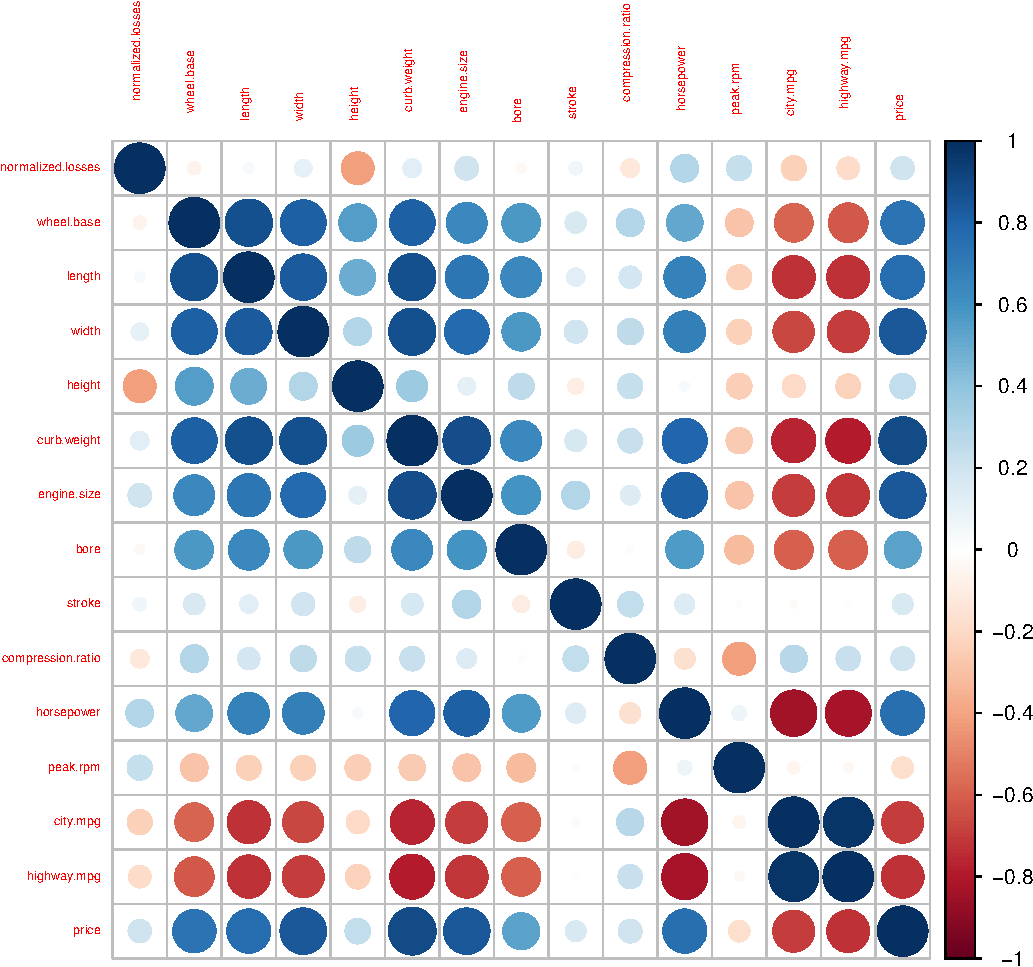
\includegraphics[width=\textwidth]{corrplot}
\caption{Correlation matrix plot.}
\label{fig:corrplot}
\end{figure}



%logarithmicTransformation
\begin{figure}[hbpt]
\centering
 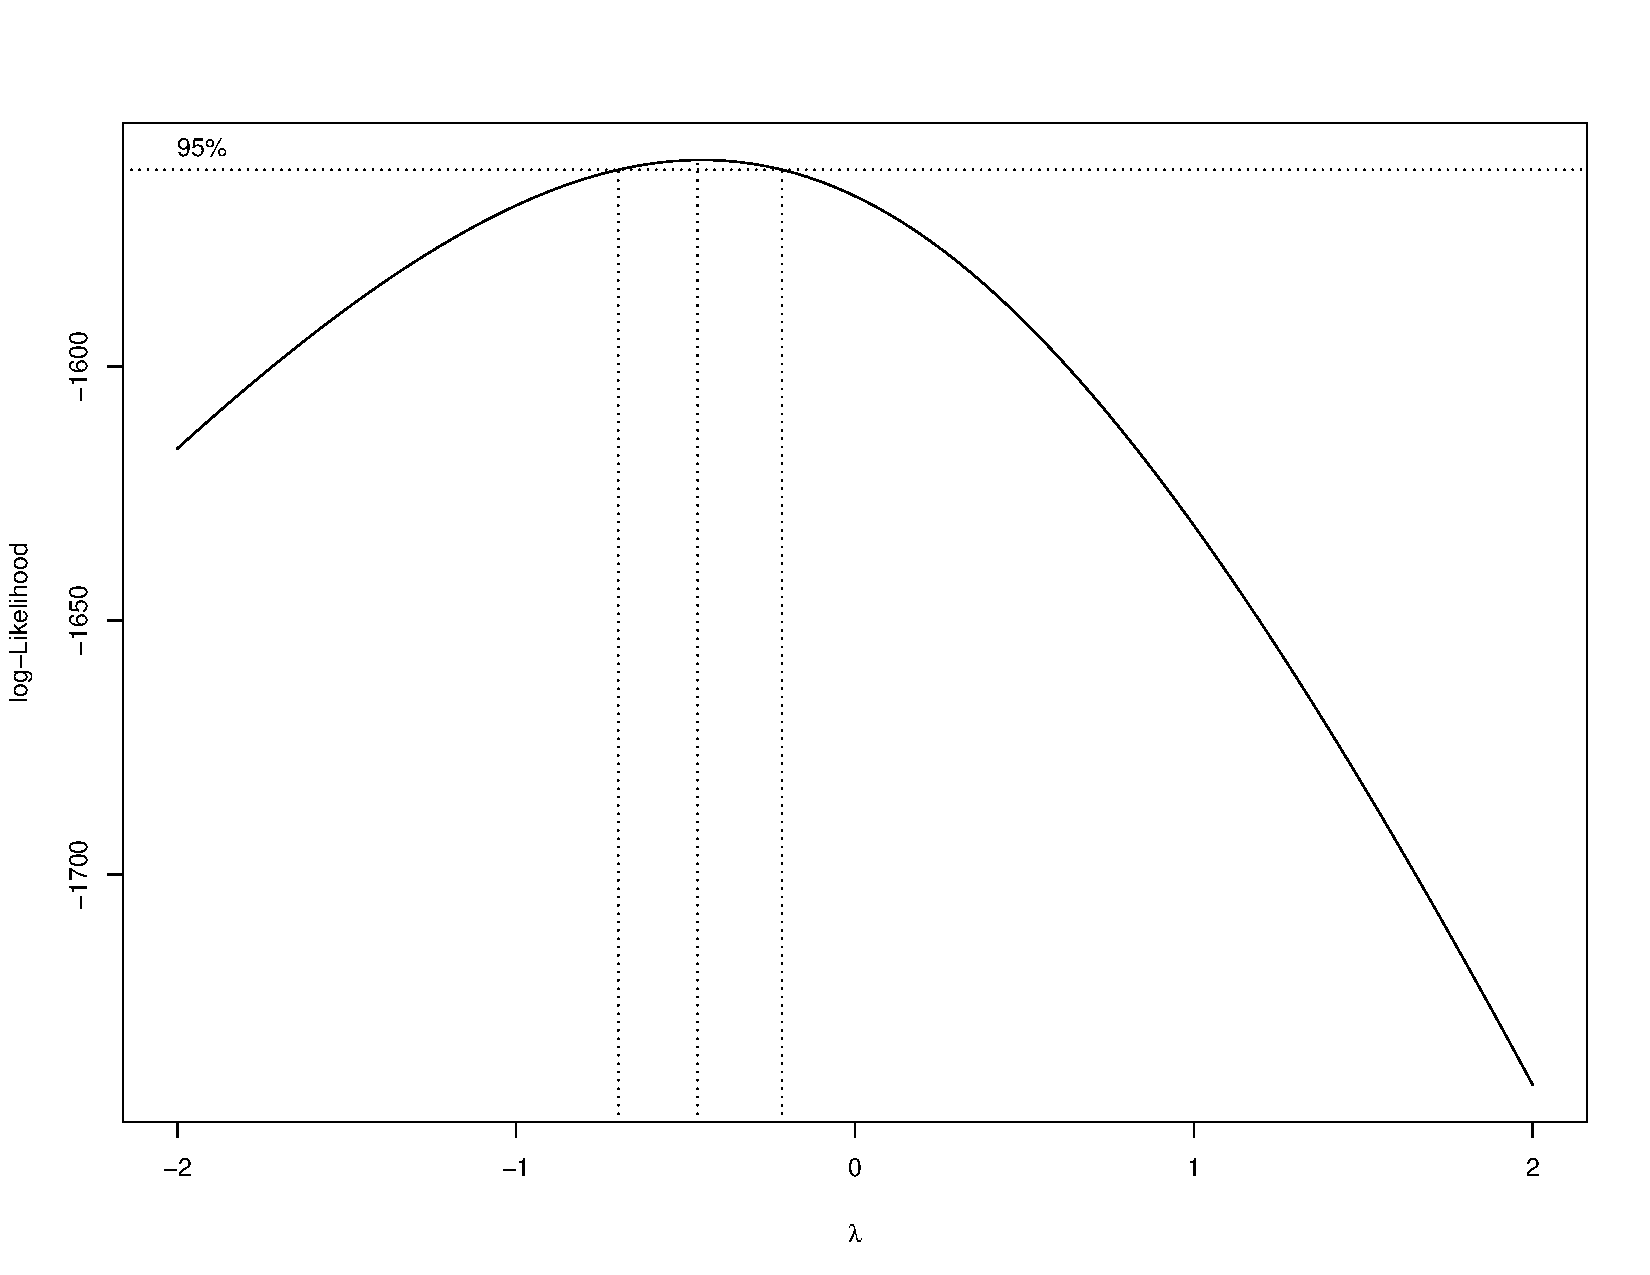
\includegraphics[width=0.65\textwidth]{boxcox}
\caption{Maximum likelihood of BoxCox transformation: $\lambda \approx -0.45$.}
\label{fig:boxcox}
\end{figure}

\begin{figure}[hbpt]
\centering
 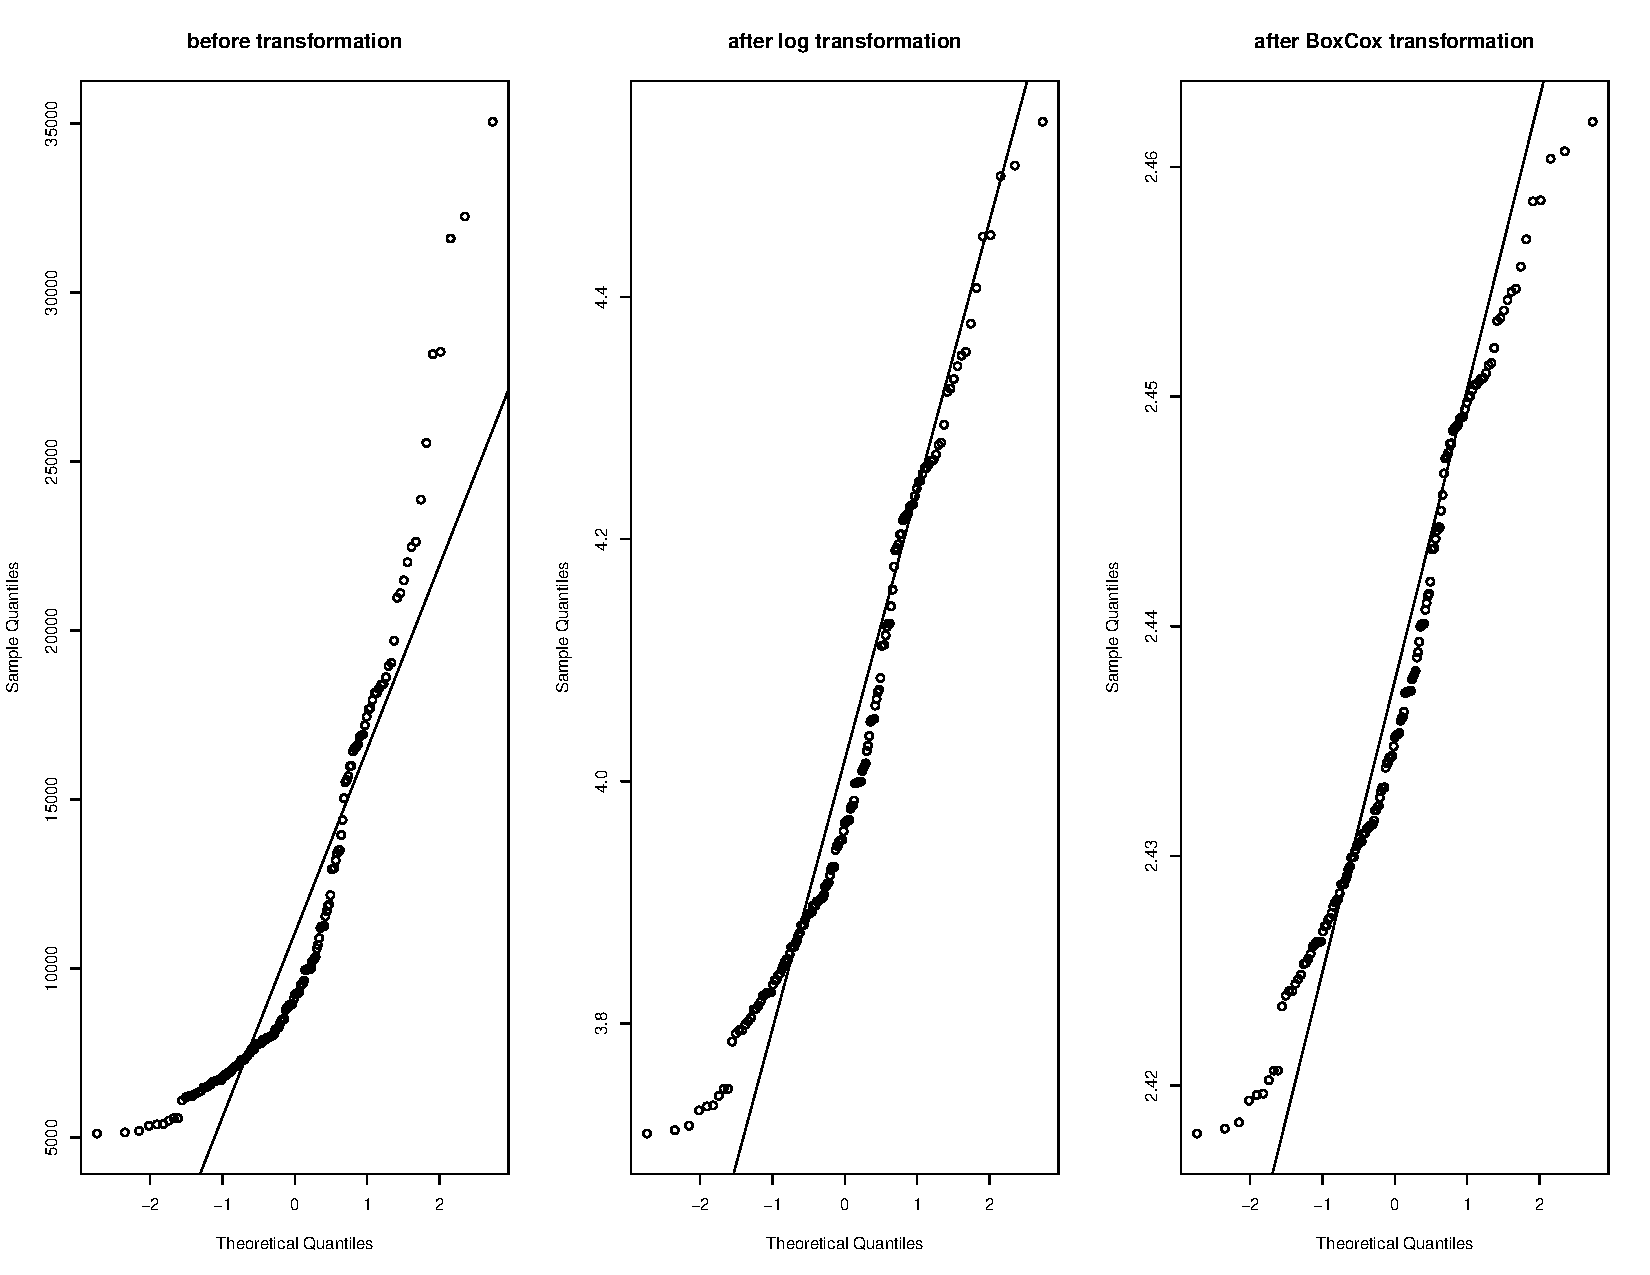
\includegraphics[width=0.85\textwidth]{logarithmicTransformation}
\caption{Transformation of the price improves normality.}
\label{fig:logarithmicTransformation}
\end{figure}

\begin{figure}[hbpt]
\centering
 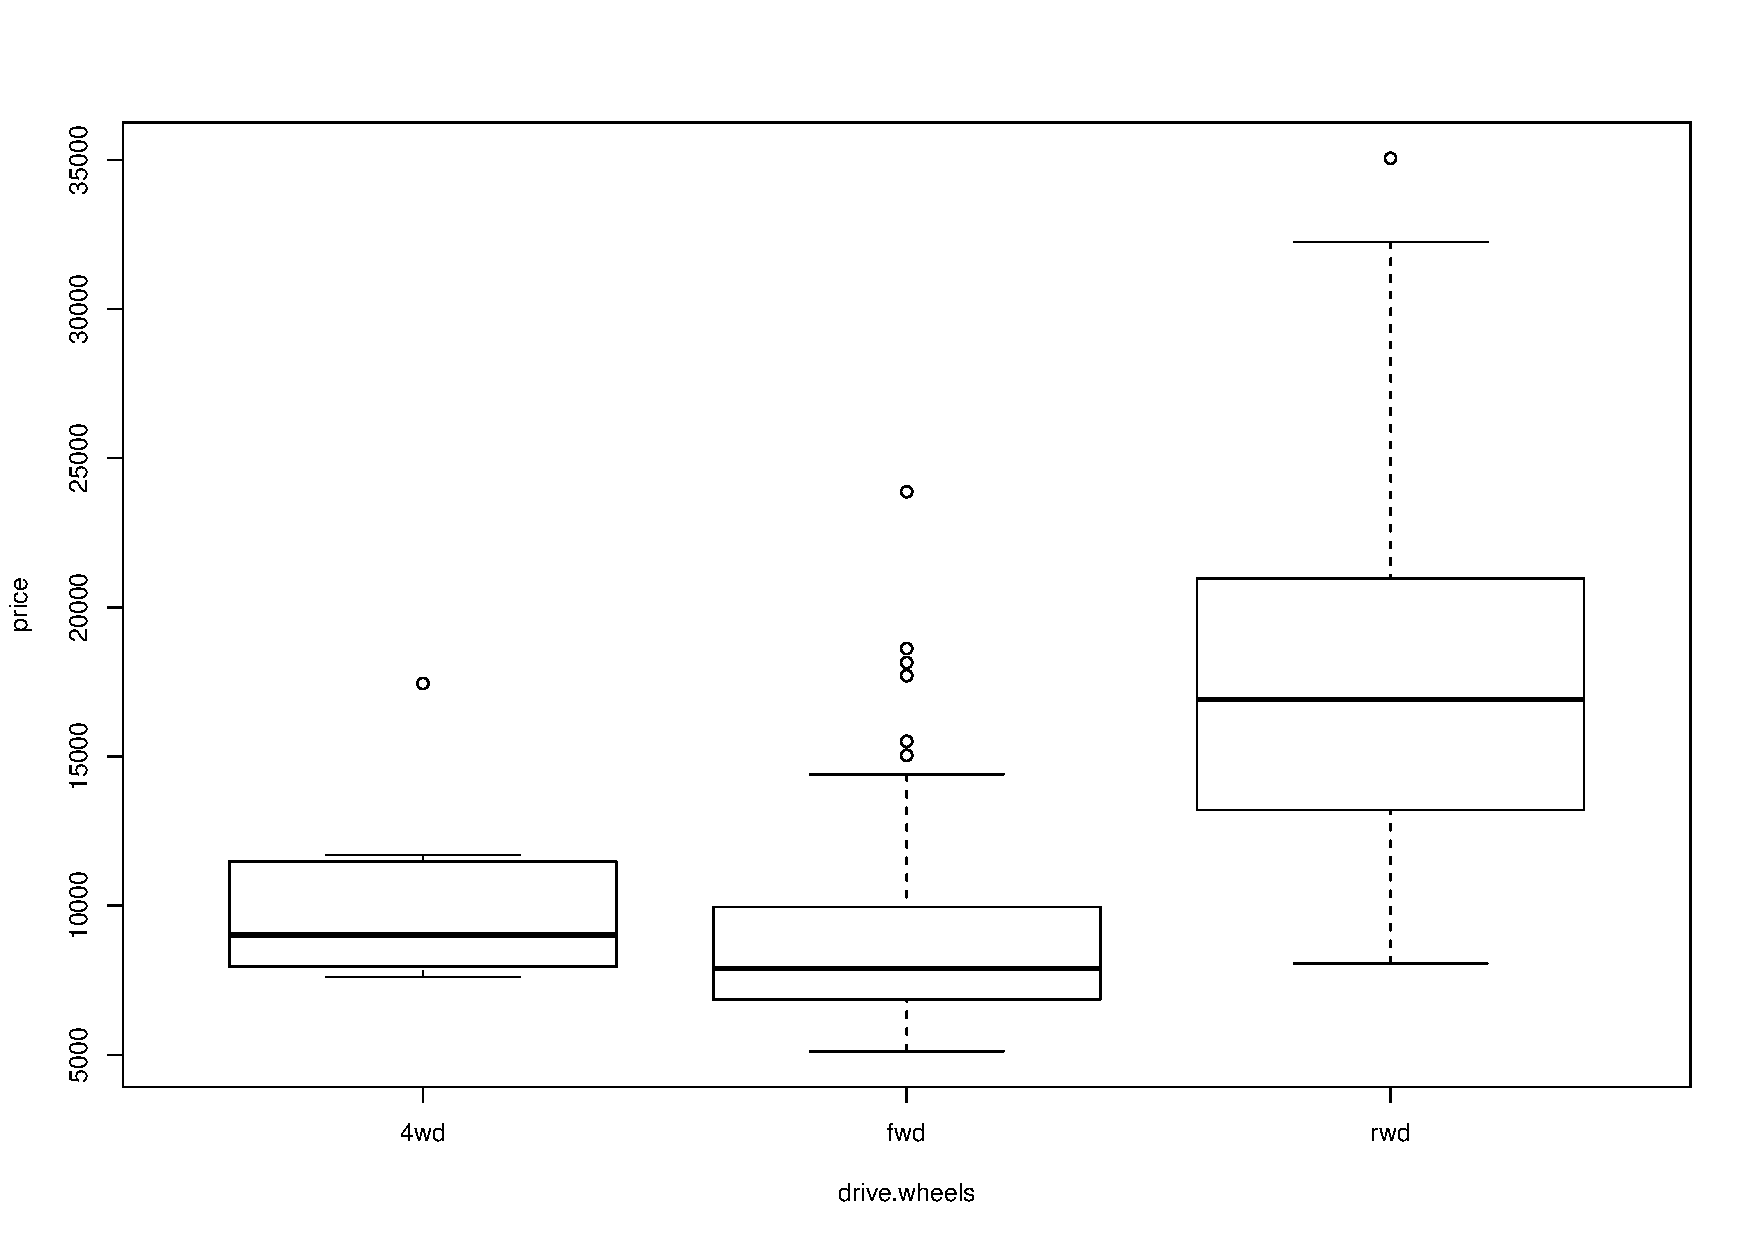
\includegraphics[width=0.95\textwidth]{boxplot_drivewheels}
\caption[Boxplot of drive-wheels versus price]{Boxplot of drive-wheels versus price---before and after BoxCox transformation.}
\label{fig:drivewheelsbox}
\end{figure}






%%PCA
\begin{figure}
  \centering
  \subfloat[Screeplot]{\label{fig:screeplot}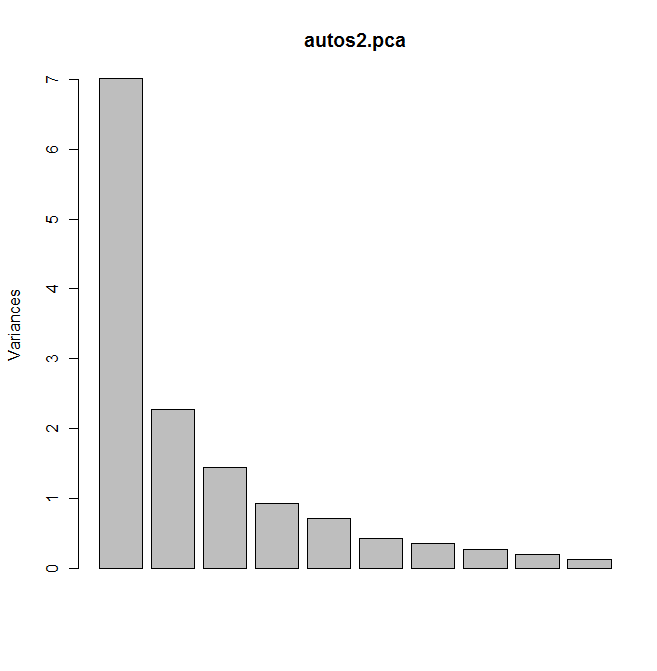
\includegraphics[width=0.5\textwidth]{pcascreeplot.png}}%screeplot}   }
  \subfloat[Biplot]{\label{fig:biplot}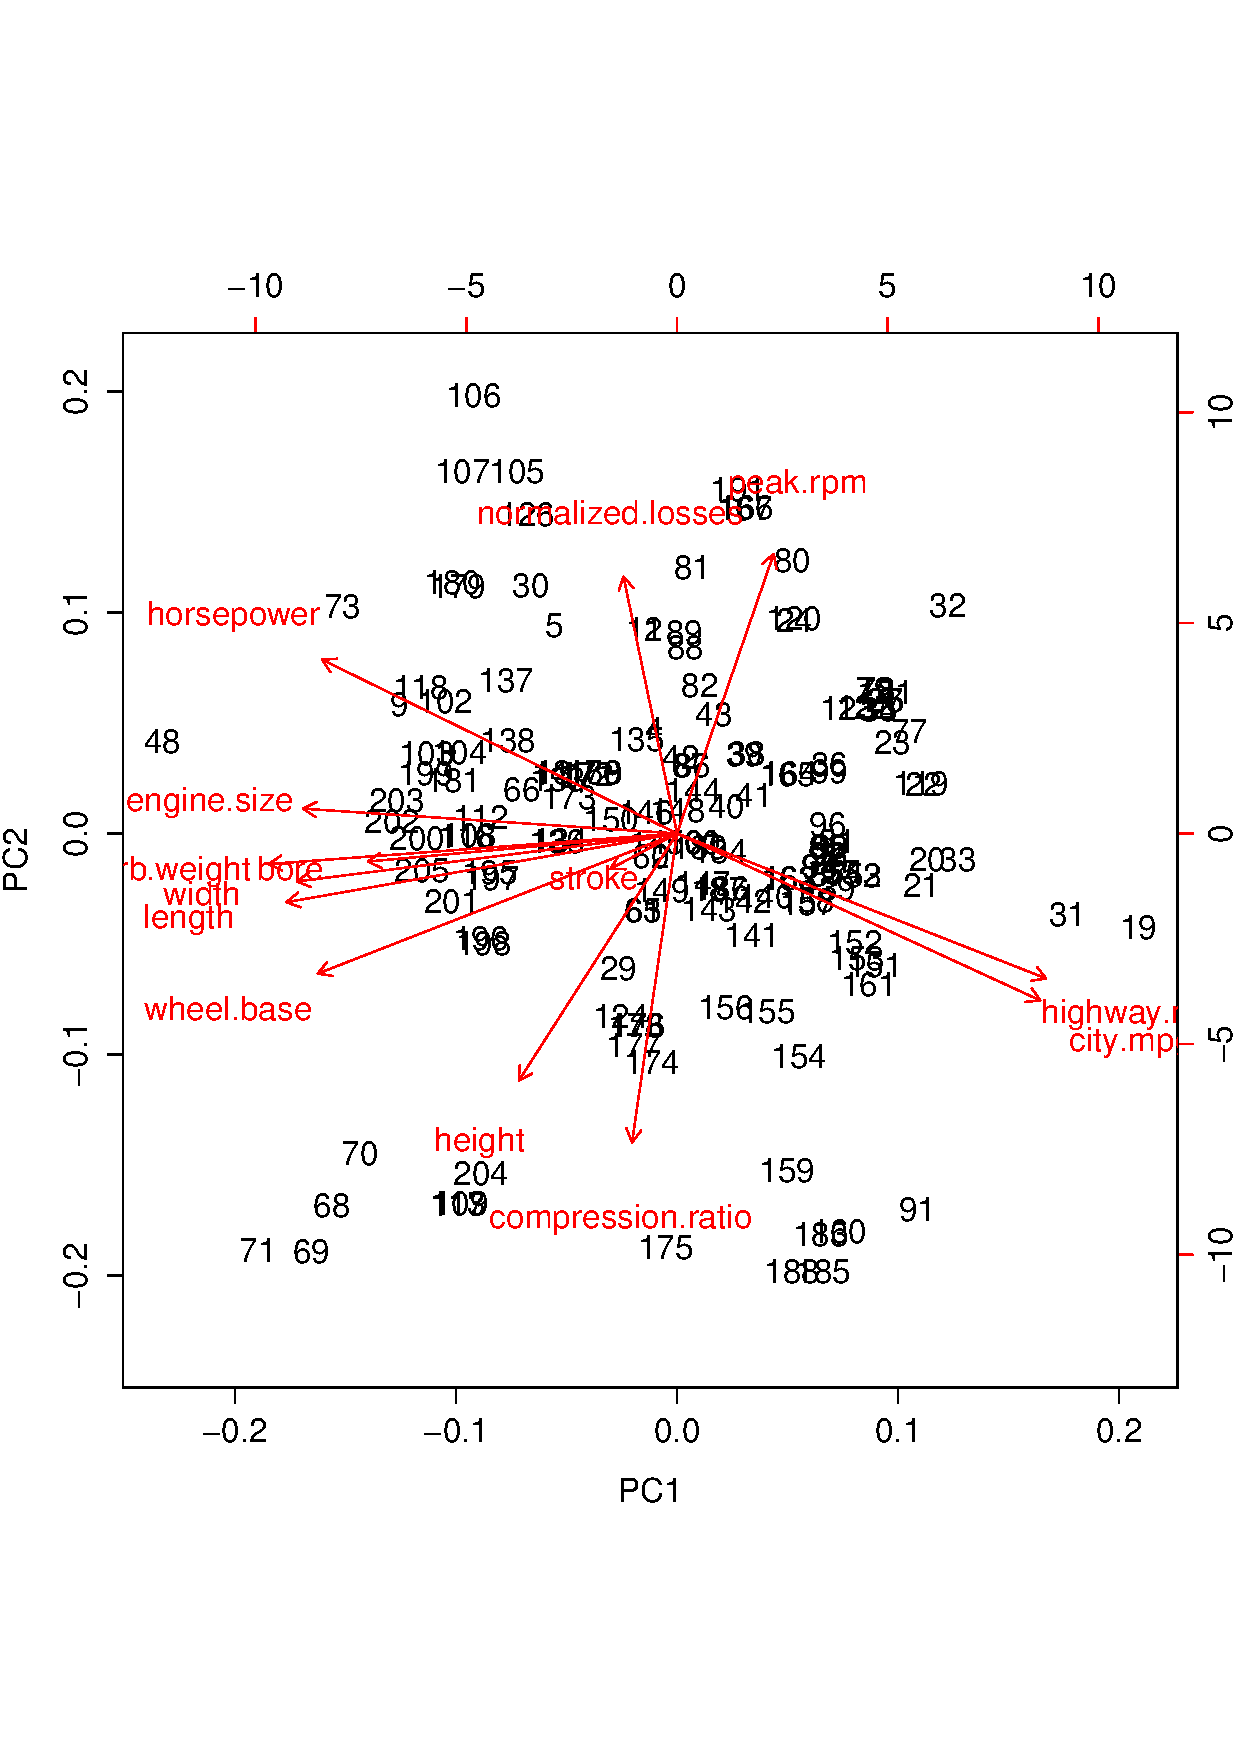
\includegraphics[width=0.5\textwidth]{biplot}}
  \caption{PCA.}
  \label{fig:pca}
\end{figure}

\begin{figure}
  \centering
  \subfloat[PCR --- normal]{\label{fig:pcrnormal}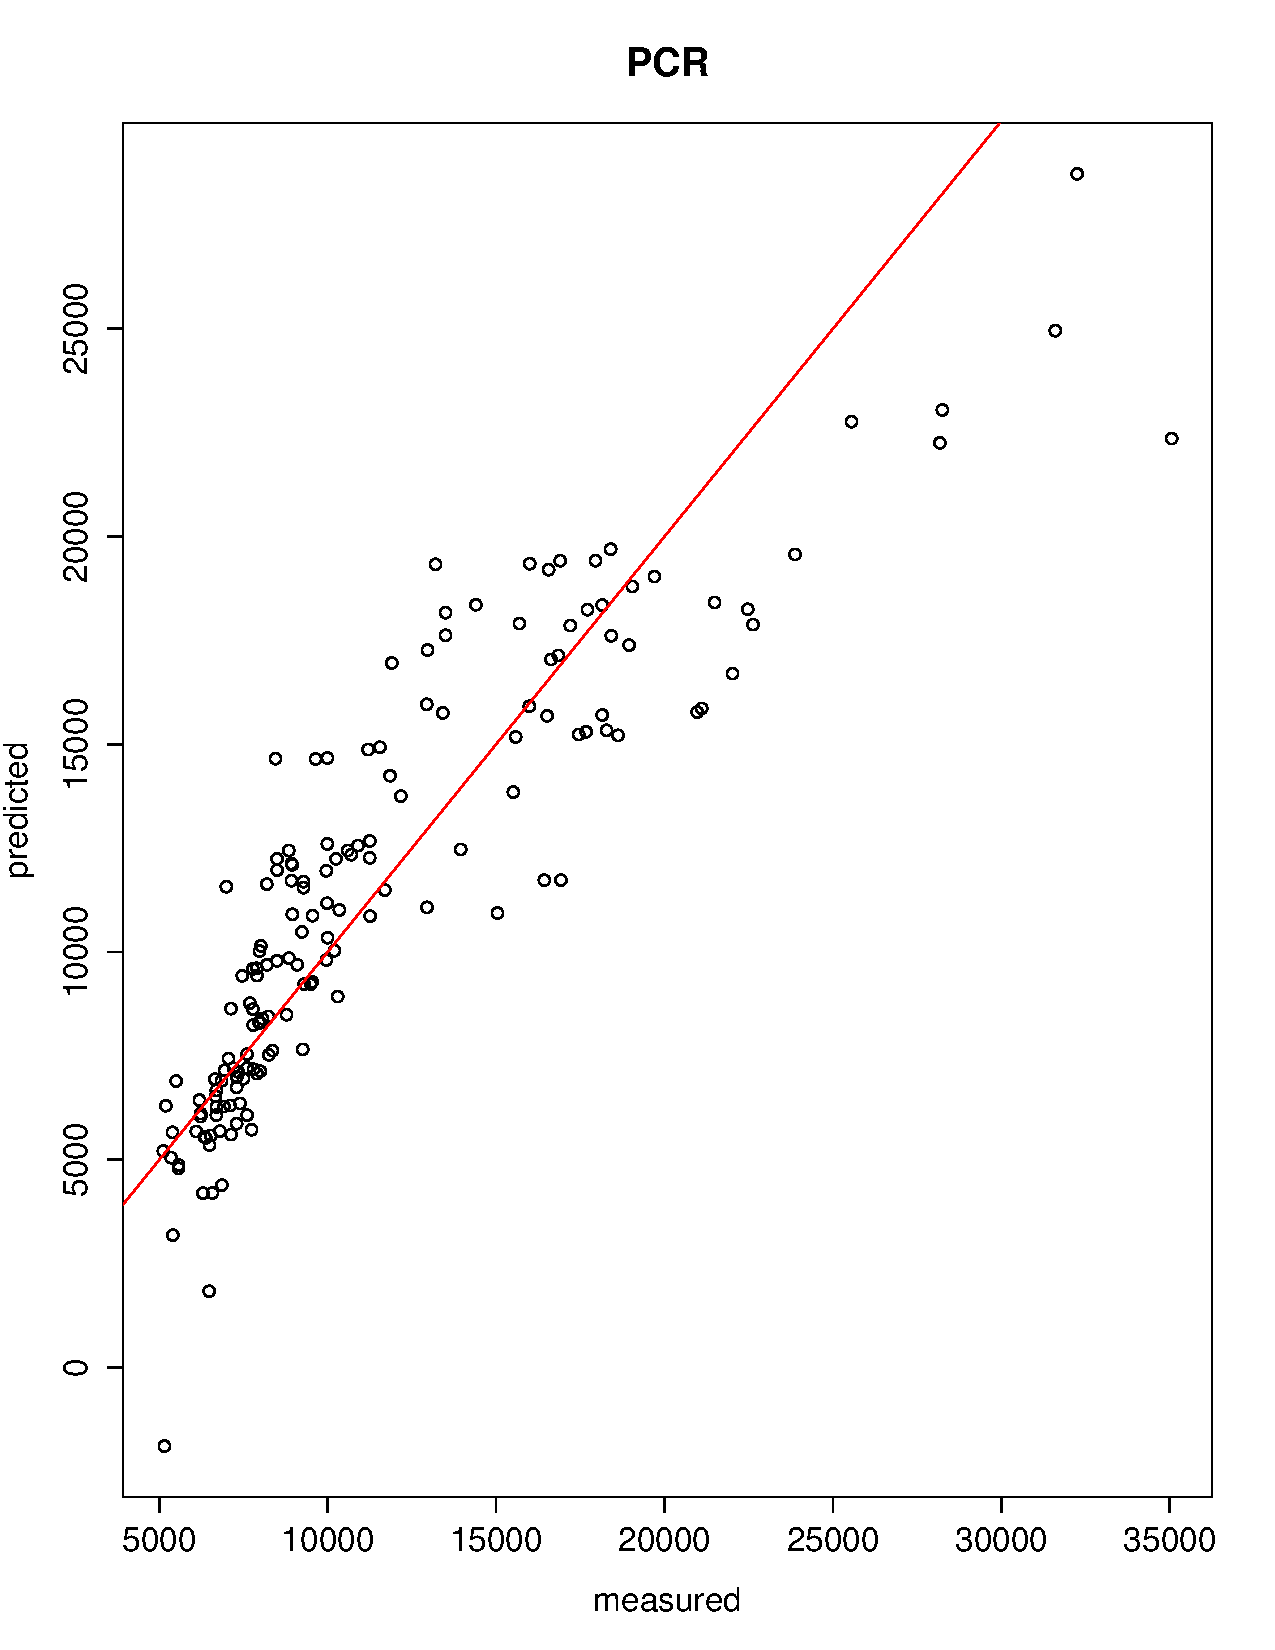
\includegraphics[width=0.5\textwidth]{PCR-pcr1.pdf}}%screeplot}   }
  \subfloat[PCR --- Box-Cox]{\label{fig:pcrbc}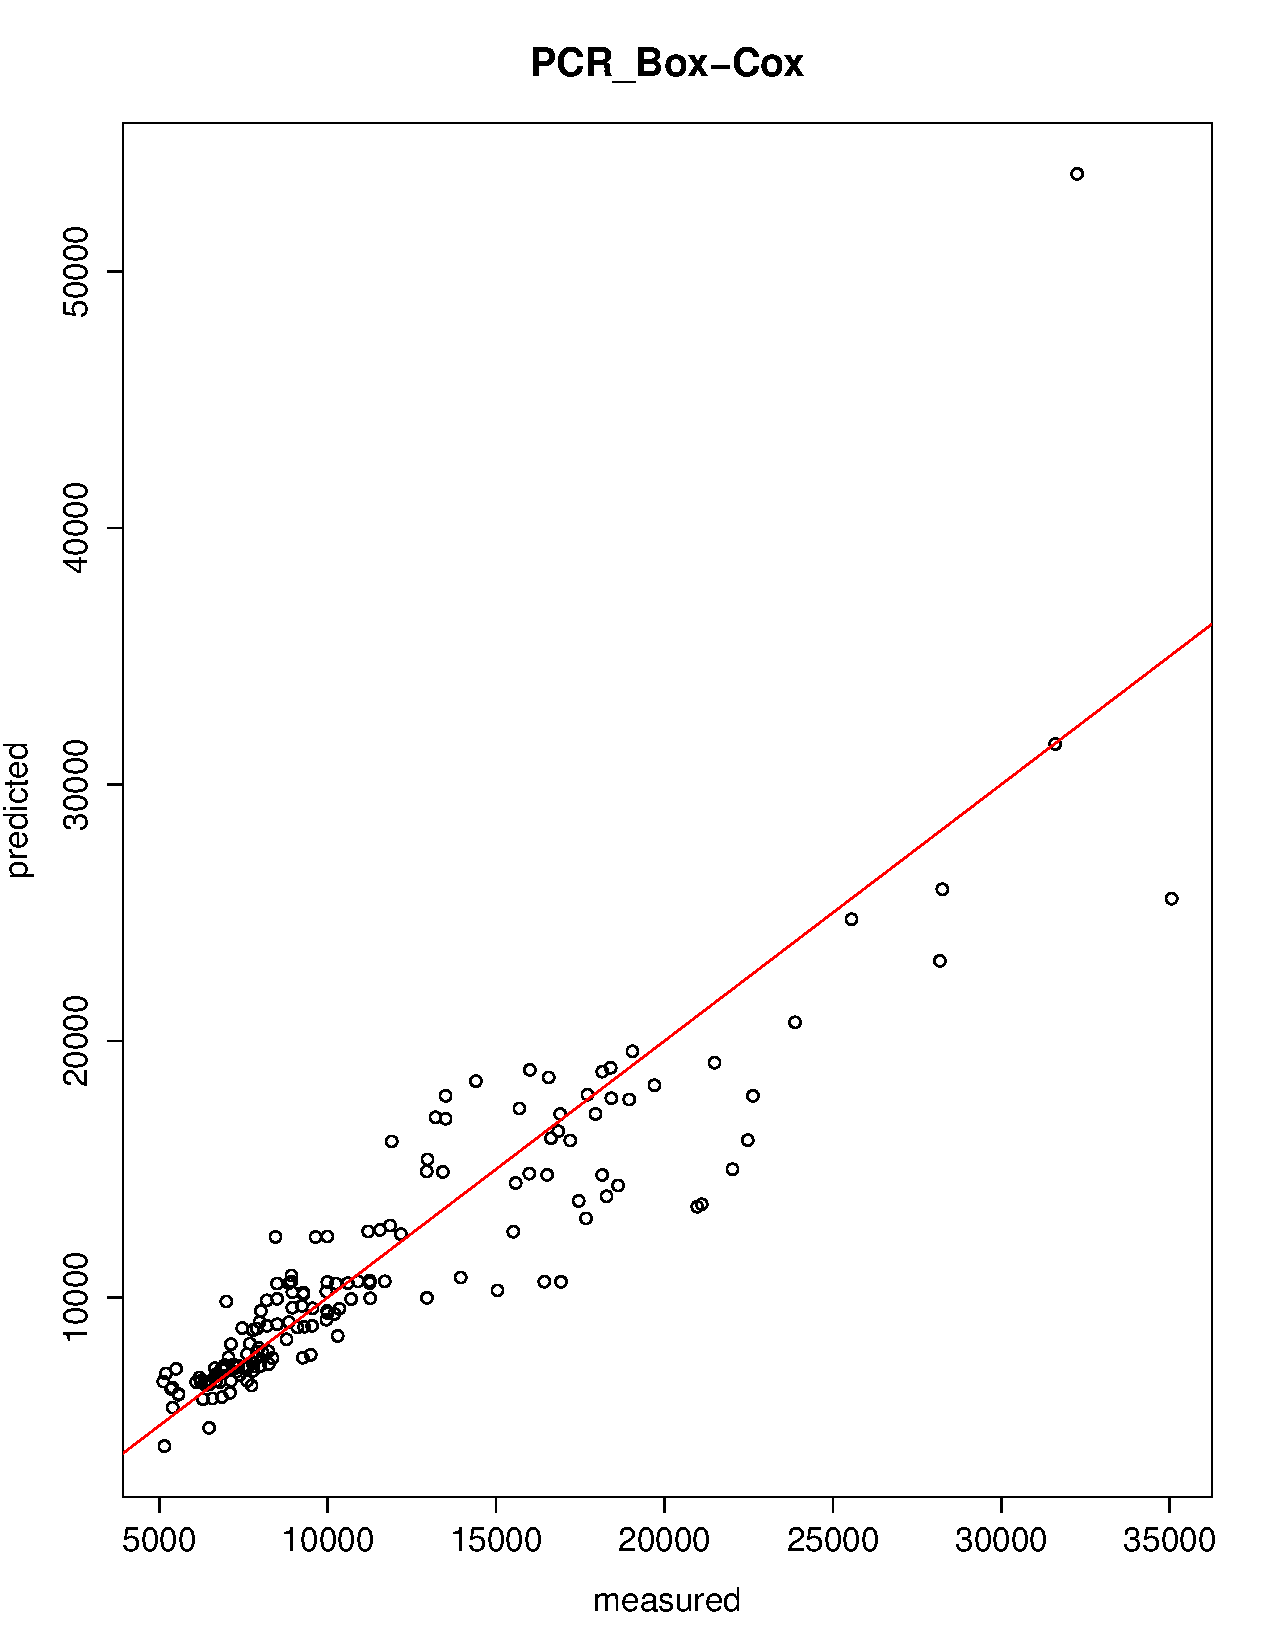
\includegraphics[width=0.5\textwidth]{PCR-boxcox.pdf}}
  \caption{PCR}
  \label{fig:pcr}
\end{figure}


\begin{figure}[hbpt]
 \centering
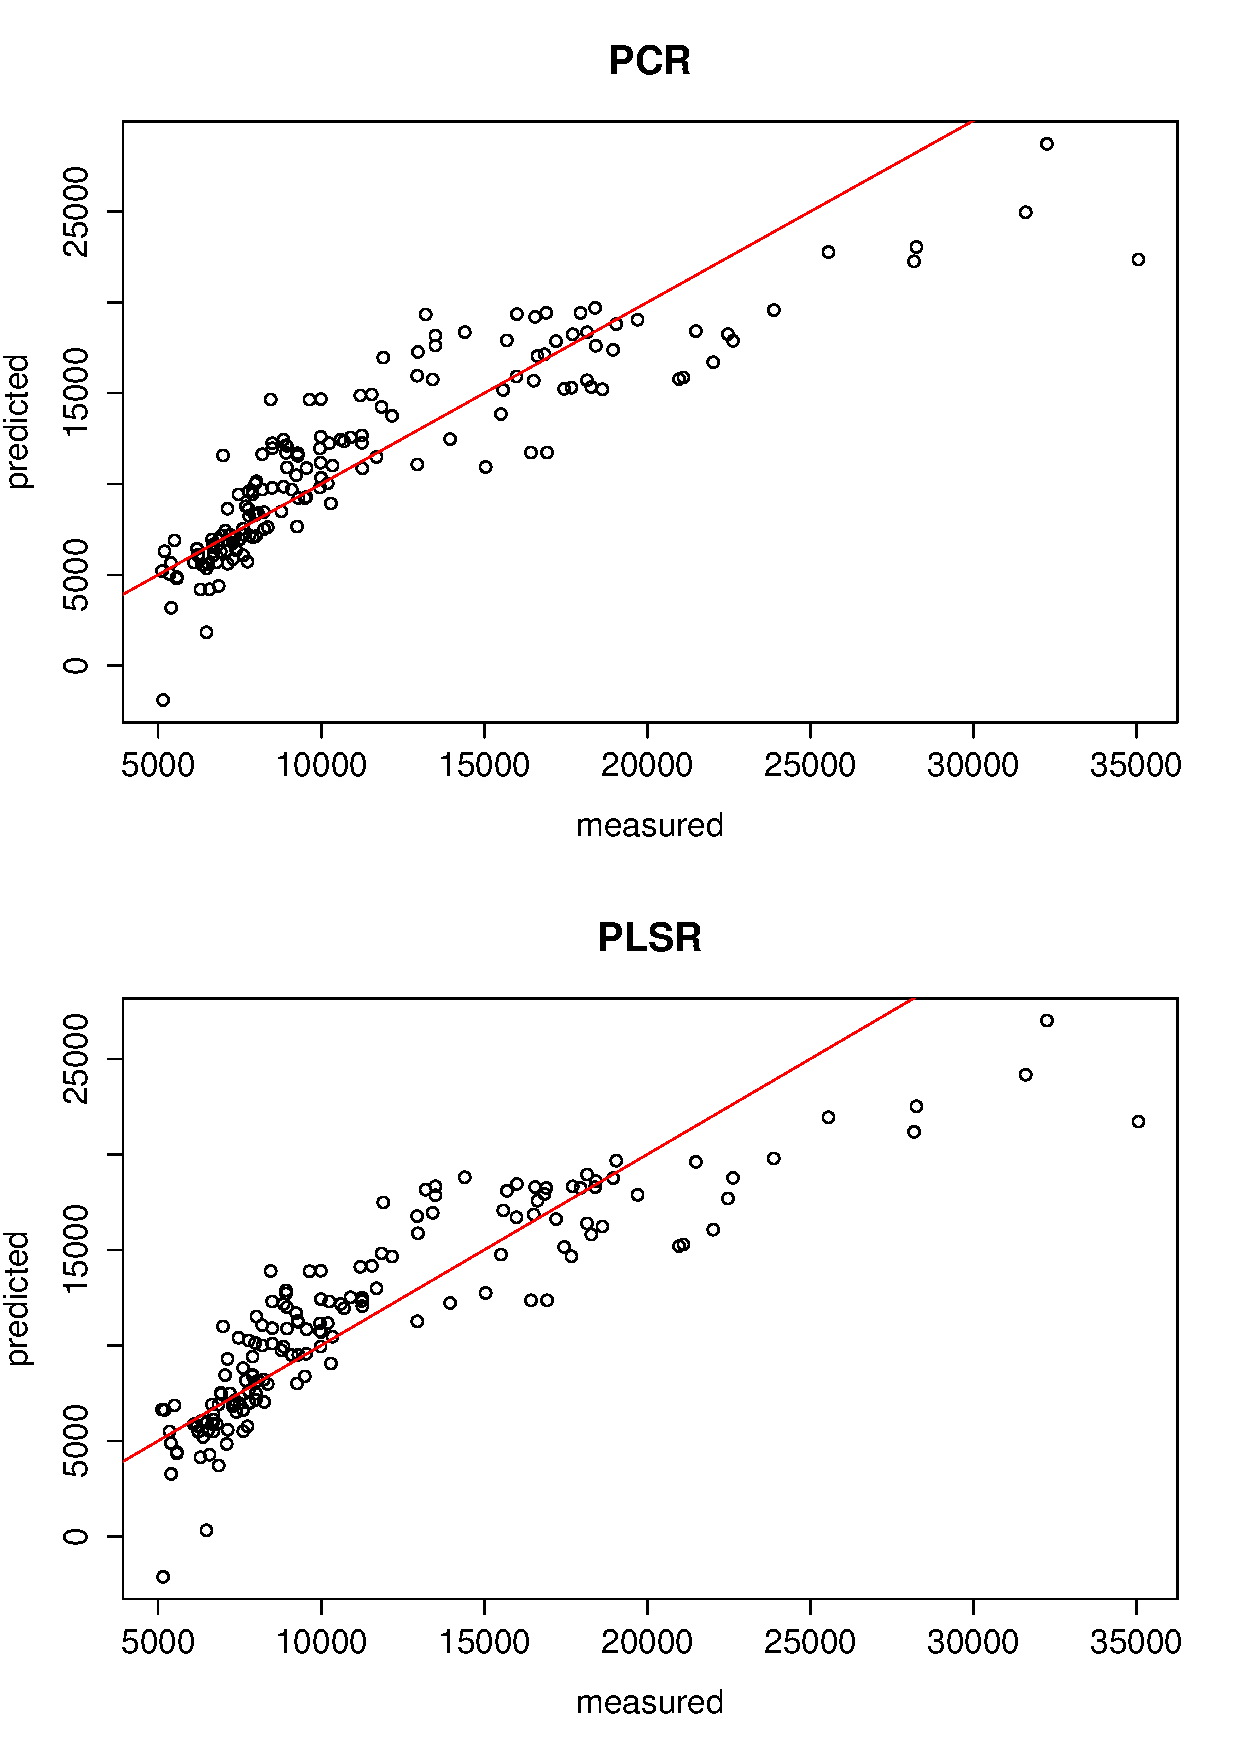
\includegraphics[width=0.95\textwidth]{PCR-PLS}%_PLS}
\caption{PCR and PLS.}
\label{fig:pcr_pls}
\end{figure}




%linear models
\begin{figure}[hbpt]
  \centering
  \subfloat[Residuals versus fitted]{\label{fig:residualsVSfitted}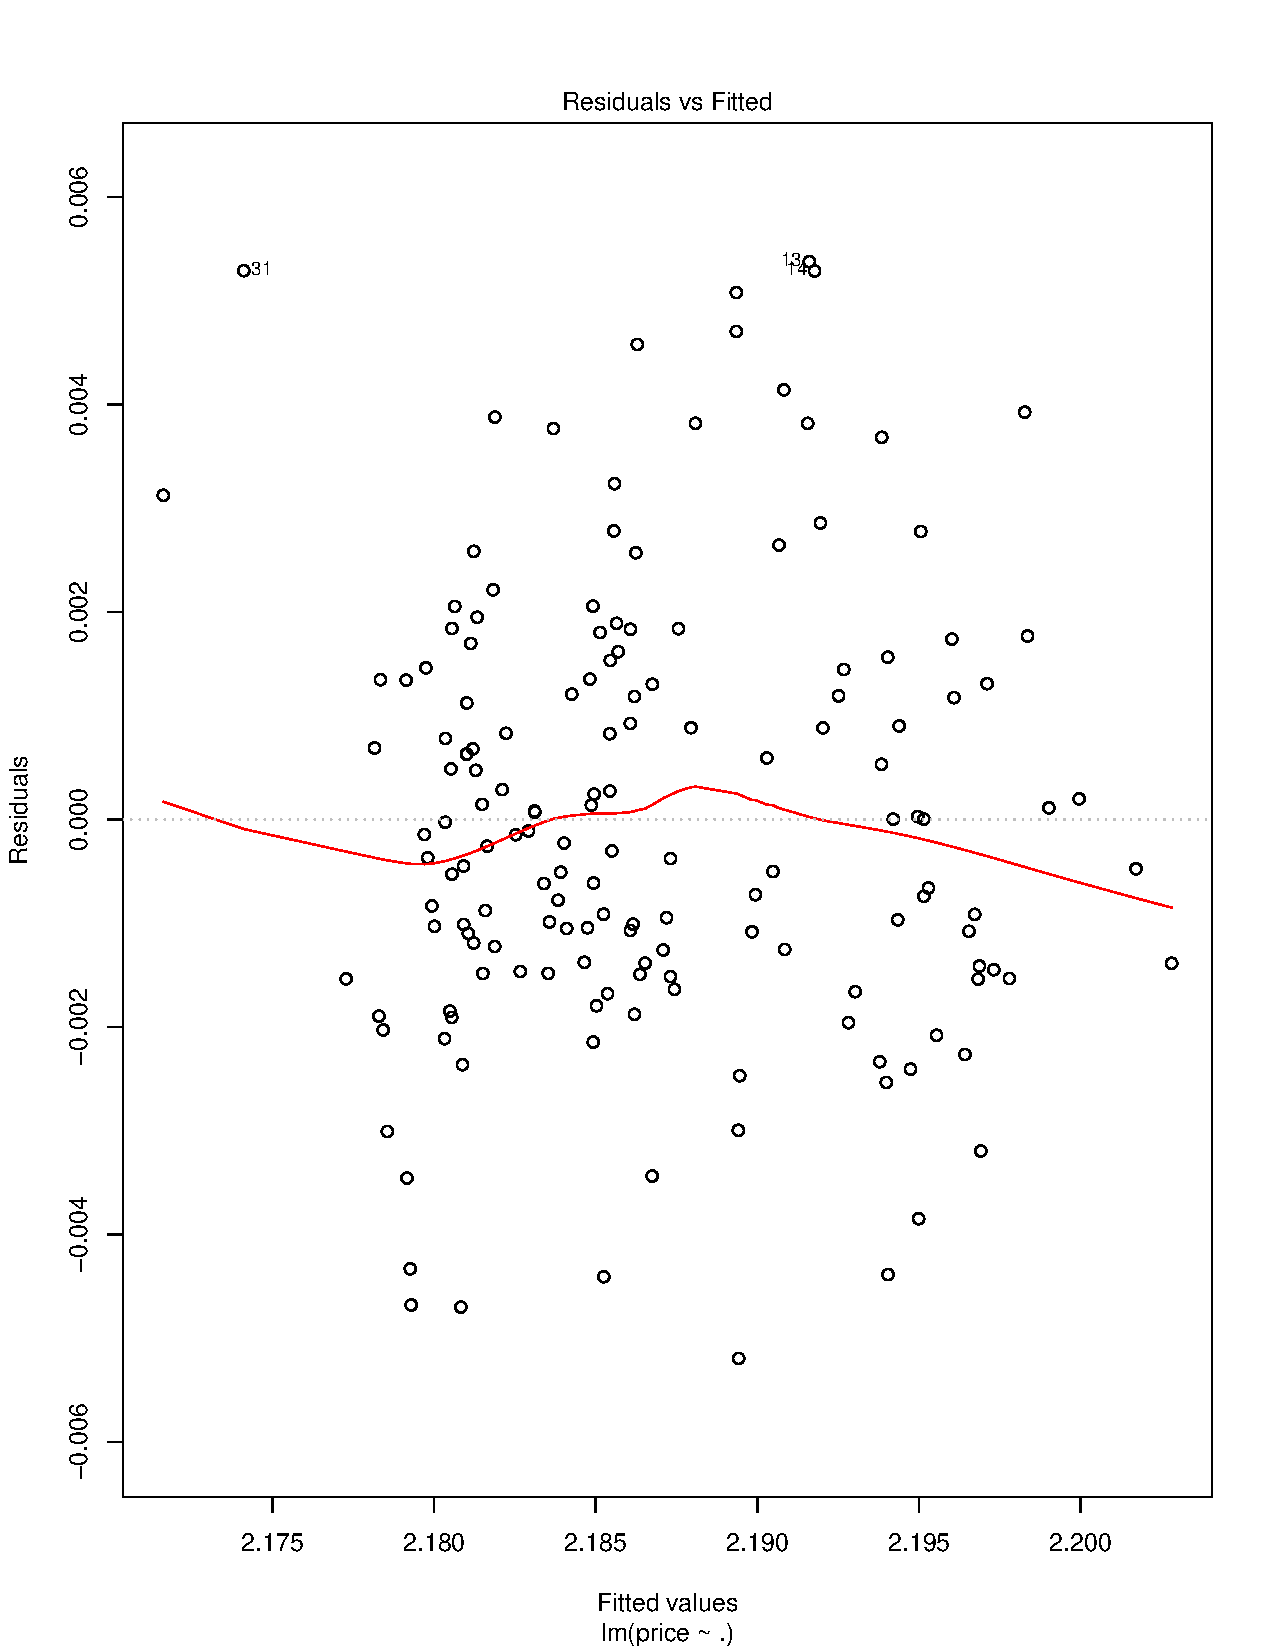
\includegraphics[width=0.5\textwidth]{residualsVSfitted}}
  \subfloat[Normal Q-Q plot of standardized residuals]{\label{fig:qqplot_residuals}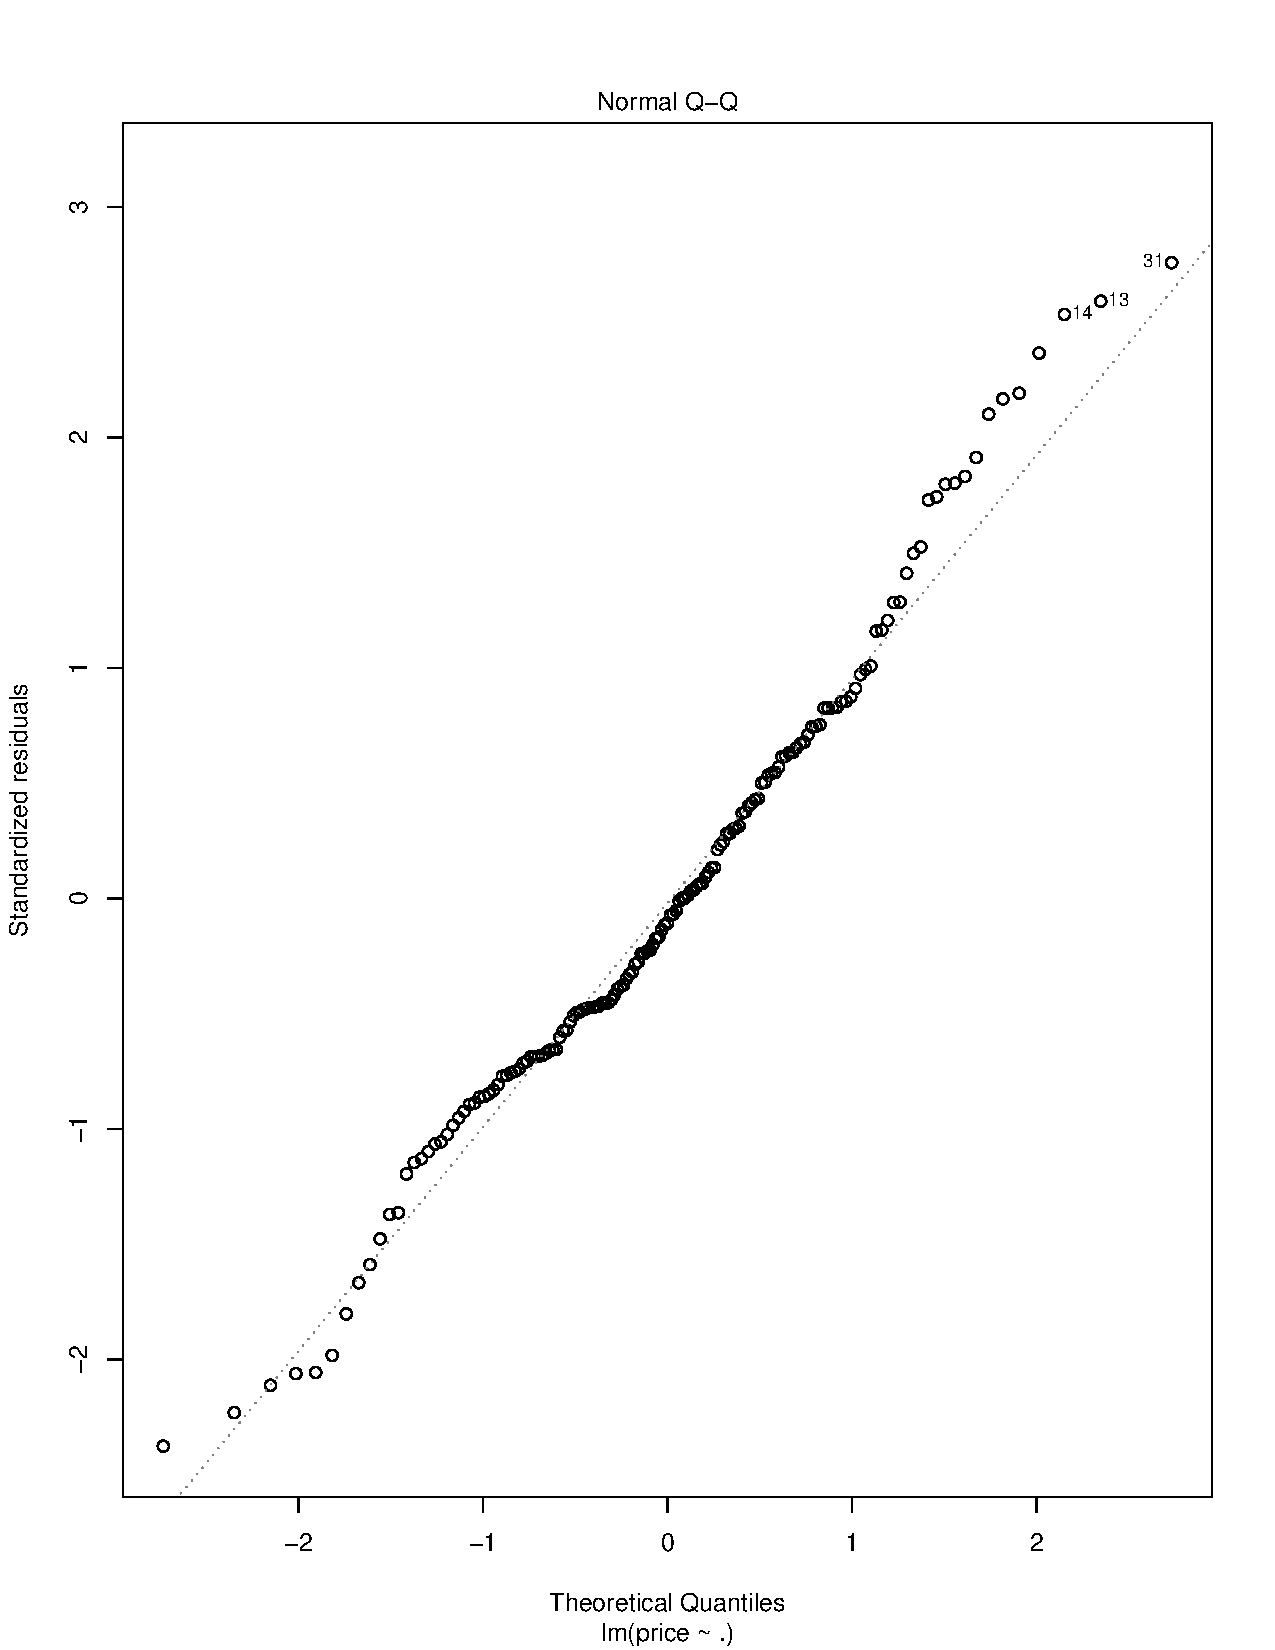
\includegraphics[width=0.5\textwidth]{qqplot_residuals}}
  \caption{Diagnostic plots for linear model using all variables as regressors.}
  \label{fig:diagnosticLM}
\end{figure}

\begin{figure}[hbpt]
  \centering
  \subfloat[Residuals versus fitted]{\label{fig:residualsVSfitted2}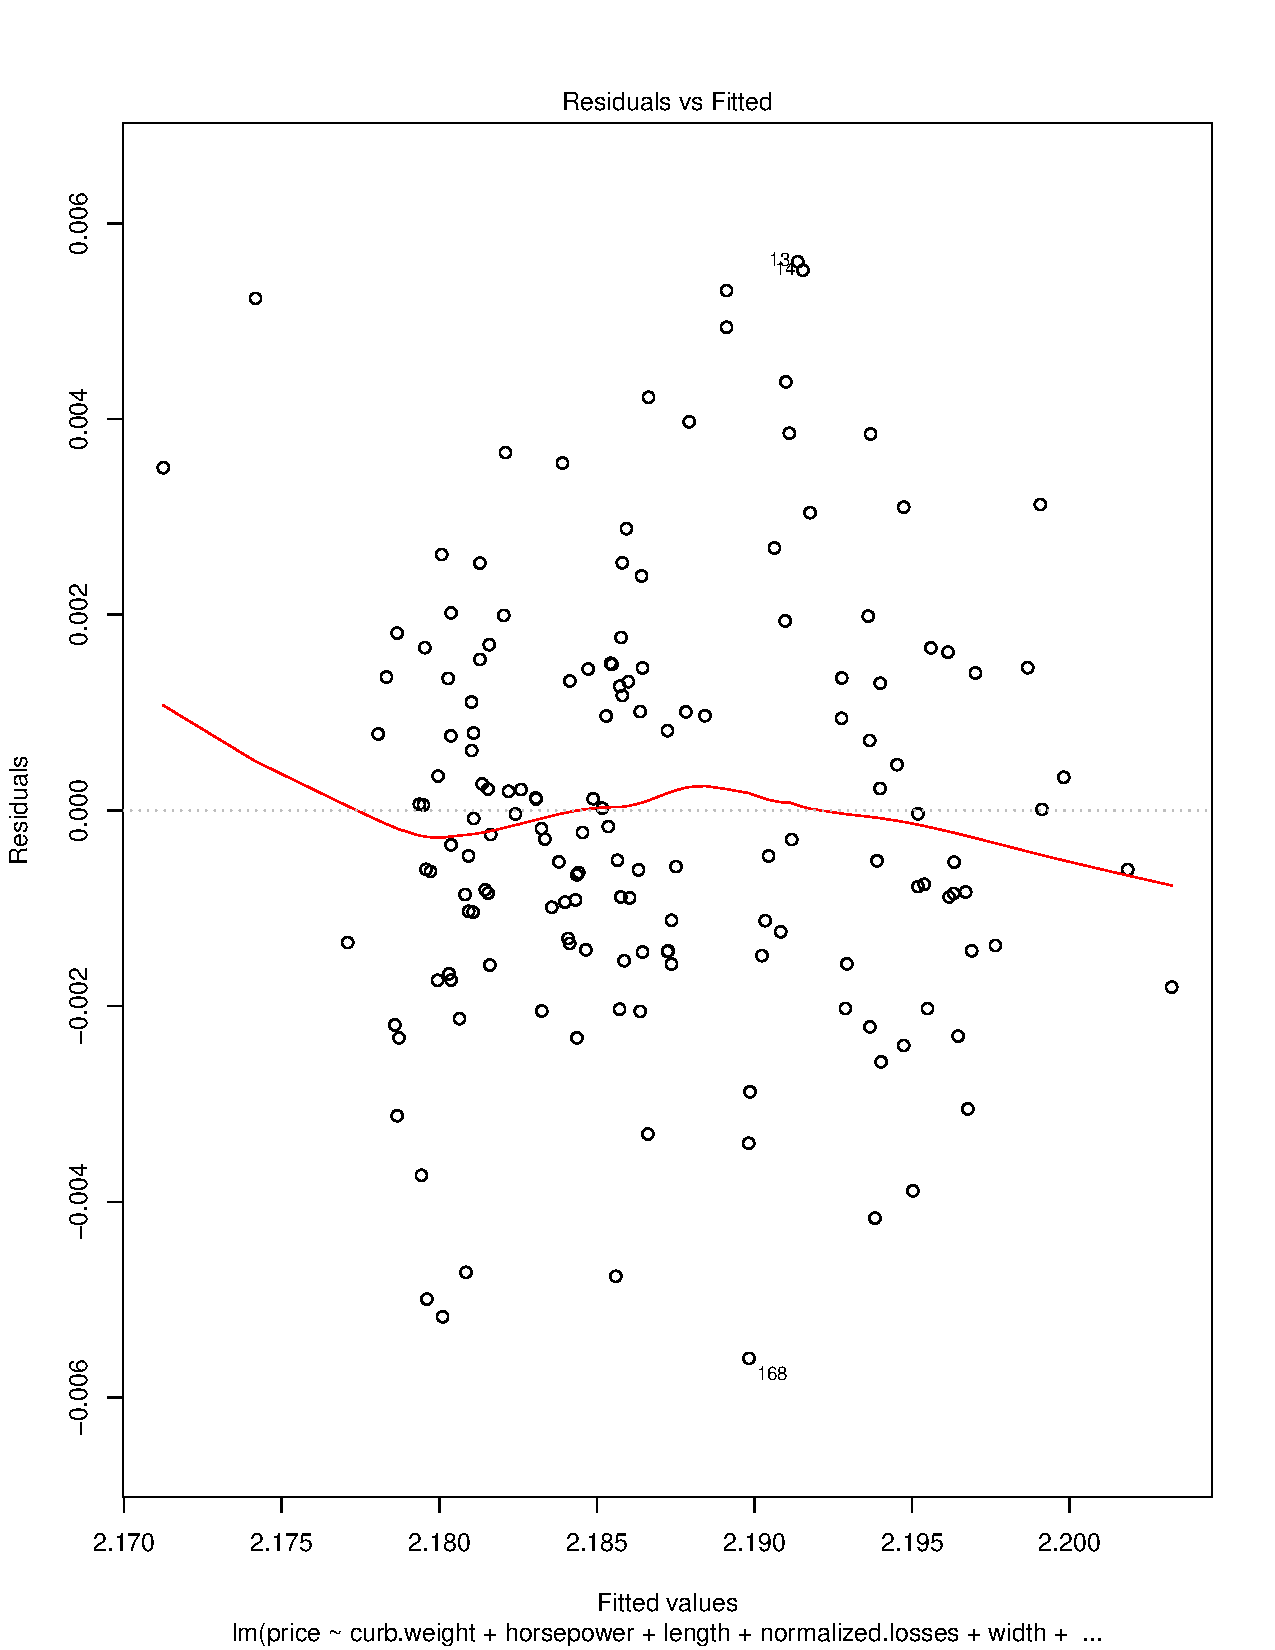
\includegraphics[width=0.5\textwidth]{residualsVSfitted2}}
  \subfloat[Normal Q-Q plot of standardized residuals]{\label{fig:qqplot_residuals2}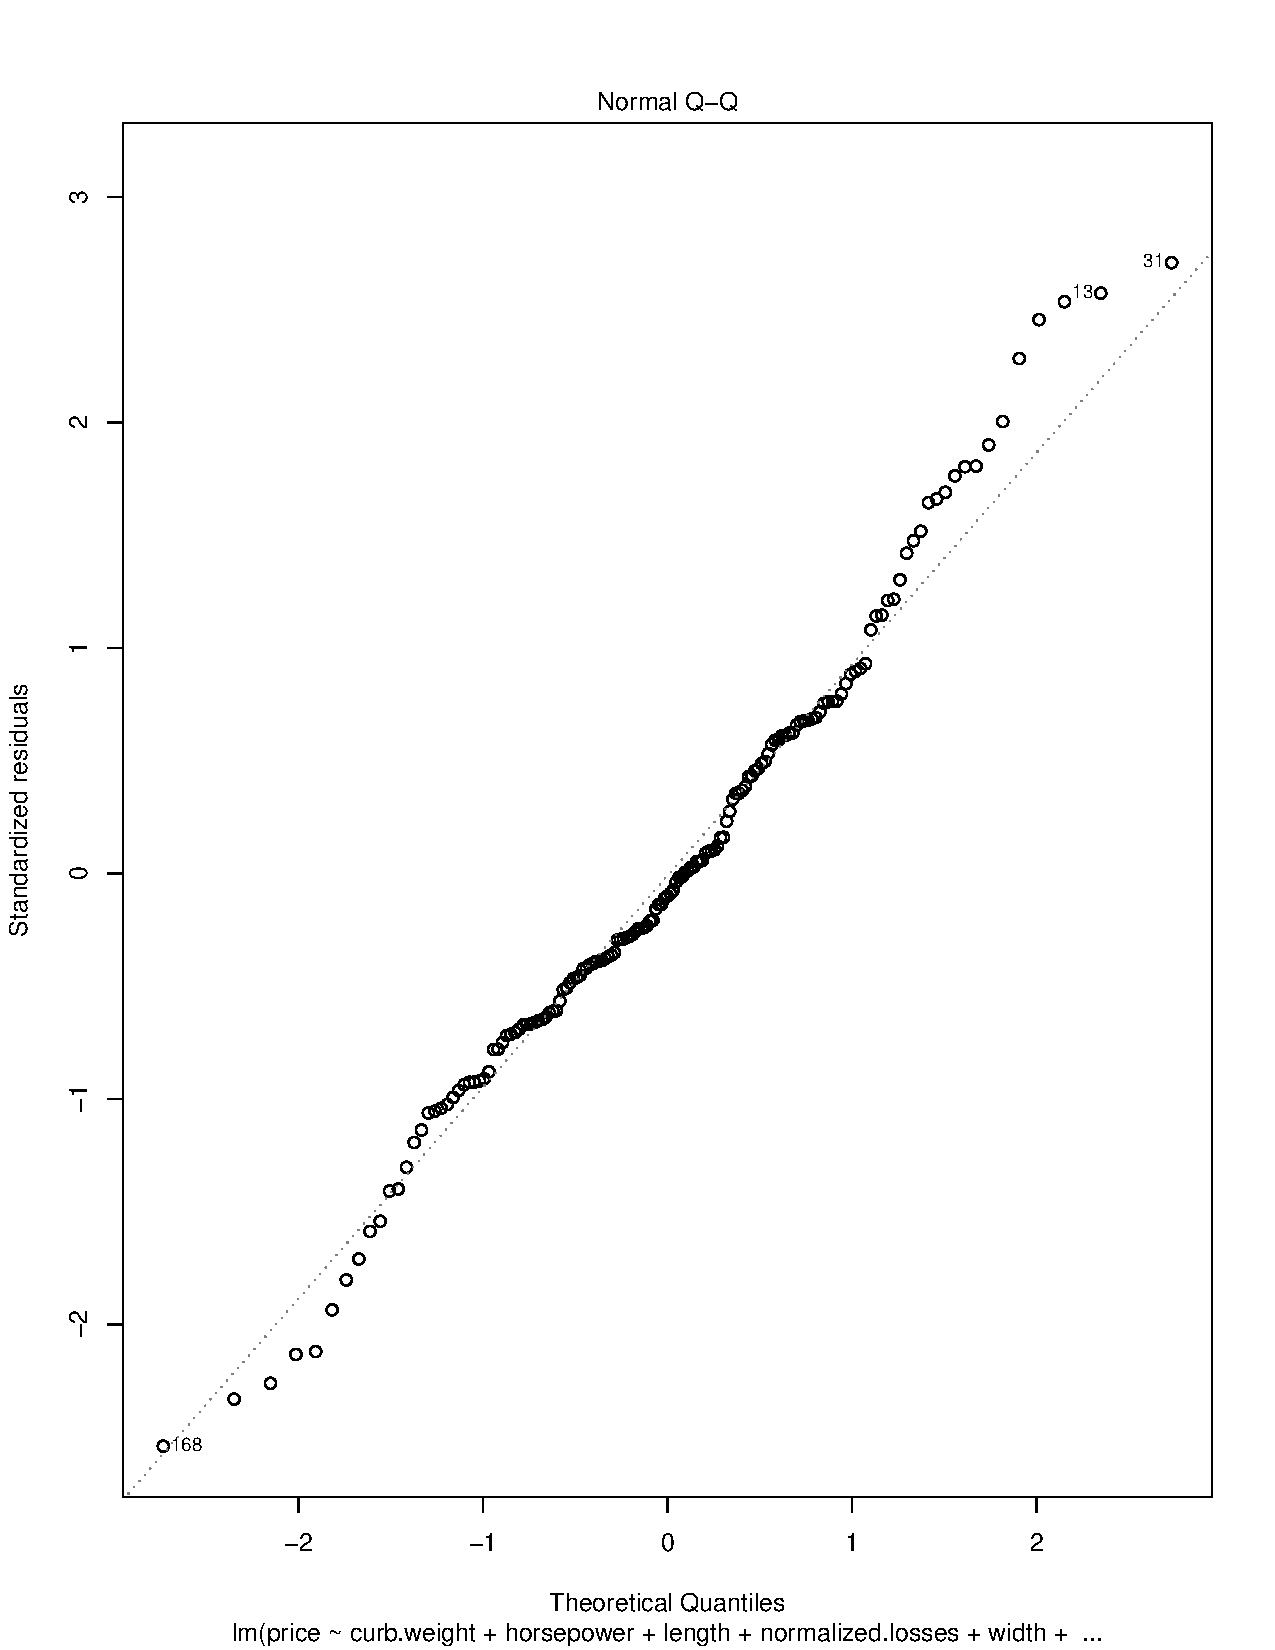
\includegraphics[width=0.5\textwidth]{qqplot_residuals2}}
  \caption{Diagnostic plots for linear model obtained by stepwise regression (AIC).}
  \label{fig:diagnosticLM2}
\end{figure}



%anova
\begin{figure}[hbpt]
 \centering
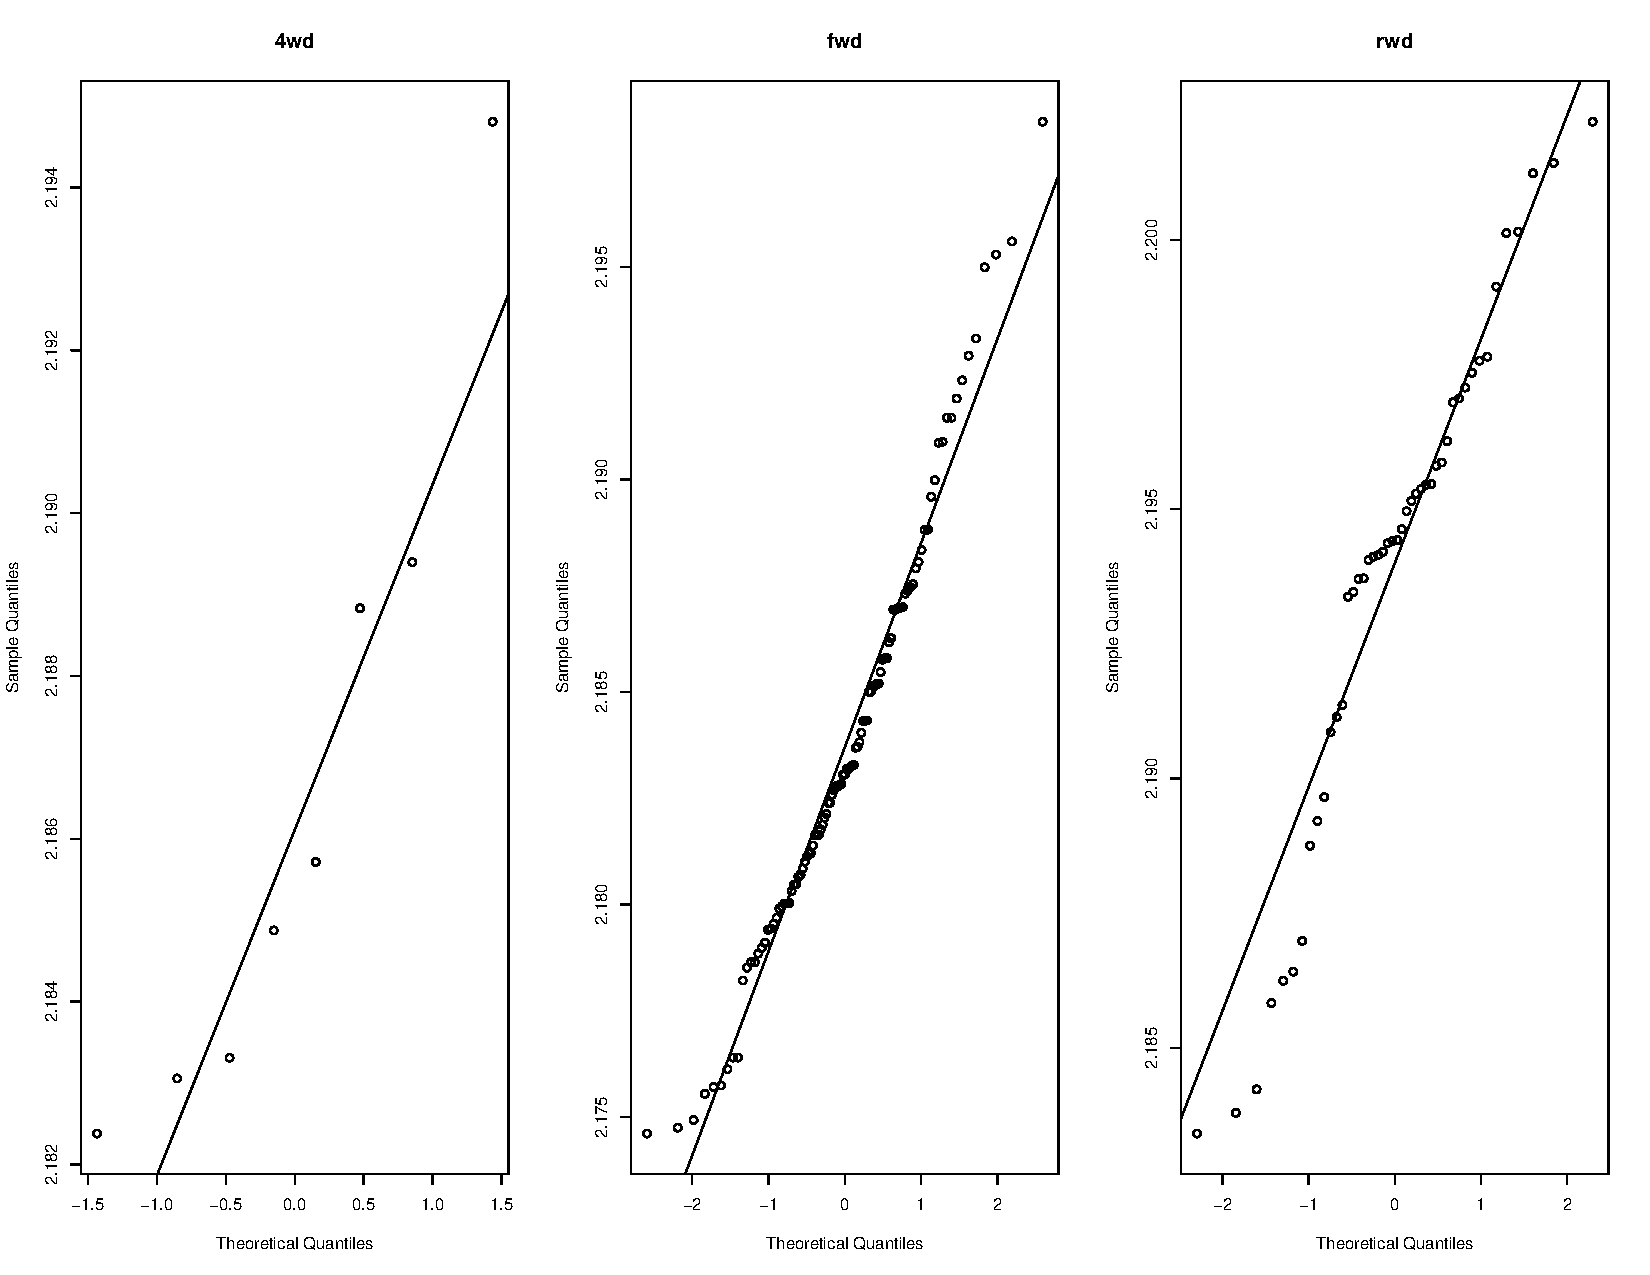
\includegraphics[width=0.95\textwidth]{normalDrivewheels.pdf}
\caption{Normal Q-Q plots of drive-wheels.}
\label{fig:qqdrive-wheel}
\end{figure}




